%%
% このファイルは,筑波大学情報学群情報メディア創成学類の
% 卒業研究論文本体のサンプルです.
% このファイルを書き換えて,この例と同じような書式の論文本体を
% LaTeXを使って作成することができます.
% 
% PC環境や,LaTeX環境の設定によっては漢字コードや改行コードを
% 変更する必要があります.
%%
\documentclass[a4paper,11pt]{jreport}

%%【PostScript, JPEG, PNG等の画像の貼り込み】
%% 利用するパッケージを選んでコメントアウトしてください.
%%
%% 推奨: graphicx パッケージ(本ファイルではこれを使用)
%%	動かない場合にいは \usepackage[dvipdfmx]{graphicx} のように dvi 変換コマンドを明示指定する.
%%
% \usepackage{graphicx} % for 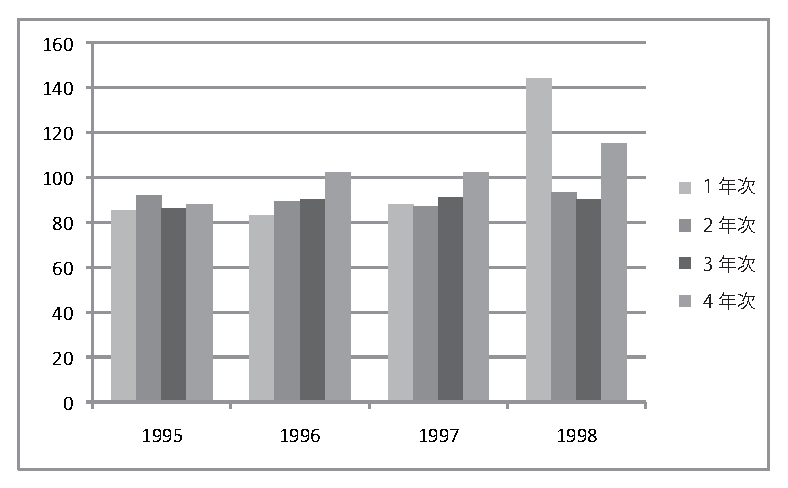
\includegraphics[width=3cm]{sample.eps}
% \usepackage[dvipdfm]{graphicx} % 画像の挿入に必要
\usepackage[dvipdfmx]{graphicx}
\usepackage[dvipdfmx]{color}
\usepackage{float} % 図の位置の強制指定に必要
%% 一応 OK (epsfig.sy)
% \usepackage{epsfig} % for 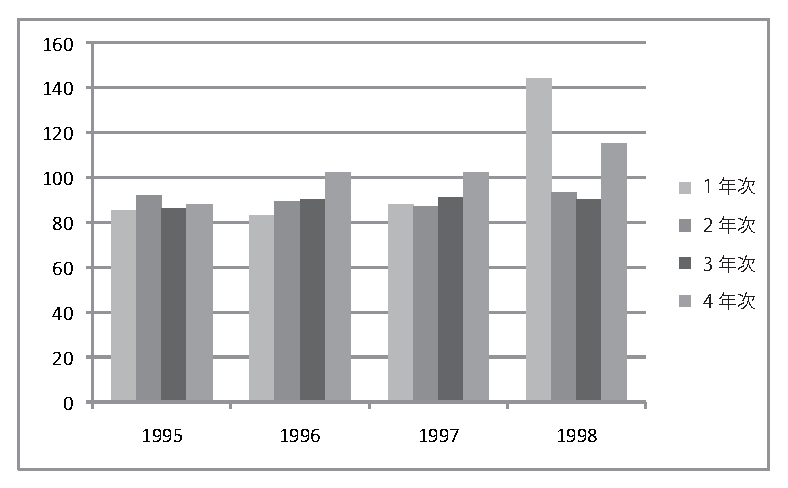
\psfig{file=sample.eps,width=3cm}
%% 以下の2つの使用はあまり勧められない (epsf.sty, epsfbox.sty)
%\usepackage{epsf} % for \epsfile{file=sample.eps,scale=0.6}
%\usepackage{epsbox} % for \epsfile{file=sample.eps,scale=0.6}

\usepackage{times} % use Times Font instead of Computer Modern
\usepackage{mdframed}
\usepackage{latexsym} % 数式で使える記号を増やす
\usepackage{amsmath} % 数式の記述環境
\usepackage{fancyhdr} % ヘッダとフッタの設定に必要
\usepackage{algorithm,algpseudocode} % 疑似コードの記述に必要
\usepackage{array}
\usepackage{booktabs} % For formal tables
\usepackage{listings}

\setcounter{tocdepth}{3}	% 目次を3レベル (1.2.3) まで
\setcounter{secnumdepth}{3}	% 番号付けレベル. 3: \section まで 4: \subsubsection まで
\setcounter{page}{-1}

\setlength{\oddsidemargin}{0.1in}
\setlength{\evensidemargin}{0.1in} 
\setlength{\topmargin}{0in}
\setlength{\textwidth}{6in} 
%\setlength{\textheight}{10.1in}	% ページの縦幅を変更する場合には設定する
\setlength{\parskip}{0em}
\setlength{\topsep}{0em}

%% タイトル生成用パッケージ(重要)
\usepackage{mast-jp-utf8}

%% タイトル
%% 【注意】タイトルの最後に\\ を入れるとエラーになります
\title{大規模言語モデルを用いた語用論的\\アプローチに基づく誤解可能性を考慮した\\画像情報ラベリング}
%% 著者
\author{清野 駿}
%% 指導教員
\advisor{若林 啓}

%% 年月 (提出年月)
%% 年月は必要に応じて書き替えてください.
\majorfield{ } \yearandmonth{2024年 2月}



\begin{document}
\maketitle
\thispagestyle{empty}
\newpage

\thispagestyle{empty}
\vspace*{20pt plus 1fil}
\parindent=1zw
\noindent
%%
%% 論文の概要(Abstract)
%%
\begin{center}
{\bf 概要}
\vspace{5mm}
\end{center}
本研究は,多数の画像から特定の一枚を選ぶ際に役立つ自然言語ラベルを生成する新しい手法を提案する.

現在利用されているマルチモーダルな言語モデルは,画像に適切なラベルを割り当てる能力を有するが,大量の画像に対して個々の特性を反映したラベルを作成することは依然として難しい.

この課題に対応するため,本研究では「話し手モデル」「聞き手モデル」という語用論に基づくアプローチを採用し,内省的なプロセスを通じてラベルの質を向上させる.

このモデルは,それぞれの画像の独自性を正確に捉え,適切なラベルを生成することを目指す.

本研究では提案手法とベースライン手法によって生成したラベルを用いた被験者実験を行い,各手法ごとにラベルの誤解可能性を検証することで手法の性能を比較した.

%%%%%
\par
\vspace{0pt plus 1fil}
\newpage

\pagenumbering{roman} % I, II, III, IV 
\tableofcontents
\listoffigures
%\listoftables		% 本ファイルでは省略してある

%% ここから本文
\pagebreak \setcounter{page}{1}
\pagenumbering{arabic} % 1,2,3


\chapter{はじめに}

本研究は,複数の画像に対して区別可能な自然言語のラベルを生成する「画像情報ラベリング」に注目しており,
この技術は,ロボットによる場所のナビゲーションや,
人間への情報提供の正確性を高める上で重要な役割を担っている\cite{Yin2023}.
画像キャプション生成に関する既存の研究では,
画像に基づいて自然言語のテキストを生成する手法が開発されており\cite{Farhadi2010, Vinyals2017, Dai2023},
これらの手法は特にマルチモーダルな事前学習済みの大規模言語モデルによって支えられている.
これらのモデルは,モデルの規模(パラメータ数)と訓練データの量を増やすことで,
その品質が向上し続ける傾向にある\cite{Devlin2019}.
しかしながら,これらの大規模モデルは,多数のデータの関係を考慮した処理には適しておらず,
特に複数の画像に対する区別のあるラベリングの問題において,その性能が十分に検証されていない.
似た画像の区別を目的とした画像キャプション生成の手法の研究は行われている\cite{Vedantam2017,Cohn-Gordon2018,Nie2020,Andreas2016}が,
これらの研究では画像キャプション生成モデルの訓練を行っていることから,
大規模言語モデルを活用したキャプション生成を行うことが出来ないという課題がある.

本研究の目的は,画像情報ラベリングにおいて大規模言語モデルの潜在能力を活用し,
加えて語用論的アプローチを組み合わせることにより,ラベリングの精度を向上させることにある.
語用論的アプローチとは,聞き手の解釈を考慮して誤解を避ける言語を生成する手法であり,
複数のテキスト生成タスクにおいて品質の向上をもたらすことが報告されている.

提案される手法は,以下のアプローチに基づいている.
大規模言語モデルによって生成されたラベルの中から,誤解を引き起こしやすいものを特定し,
これを再び大規模言語モデルで修正する方法である.

実験においては,複数の部屋の画像を用い,それぞれに対してラベルを生成した.
このラベルの評価にはAmazon Mechanical Turkを利用し,人間による誤解の程度を検証した.
実験結果より,テキスト長が短いラベルにおいて,提案される語用論的アプローチによって性能が改善されることが示された.
これは,語用論的アプローチが,複数の画像に対する区別可能なラベルの生成において有効であることを示唆している.

%
% 本論文では,画像に対するラベル生成における新たなアプローチを提案する.具体的には,語用論的な観点から話し手モデルと聞き手モデルを導入し,その対話を通じてラベルの改善を図る.この新たなアプローチは,生成されたラベルが画像を一意に特定できることを保証することを目的としている.また,生成したラベルの評価にはAmazon Mechanical Turkを利用し,生成されたラベルが人間にとってどの程度理解しやすいかを検証する.本論文では,提案手法とその評価結果について詳細に述べる.



% 関連研究
\chapter{関連研究}

本章では,本研究で扱う画像情報ラベリングタスクに関連する研究として,画像に基づくテキスト生成技術について\ref{sec:relwork_image_captioning}節で述べる.
また,提案手法の着想に関連する研究として,語用論的アプローチに基づく機械学習手法について\ref{sec:relwork_pragmatic_ml}節で述べる.

\section{画像に基づくテキスト生成}
\label{sec:relwork_image_captioning}
画像内容に基づくテキスト生成技術の発展は,画像キャプション生成の研究によって牽引されてきた \cite{Farhadi2010}.
特に,深層学習を用いた画像キャプション生成では,ニューラルネットワークに画像の特徴を抽出し,得られた特徴に基づいて再帰型ニューラルネットワークでテキストを生成するモデルの枠組みが用いられる \cite{Vinyals2017}.
この枠組みにおいてXuら\cite{Xu2015}は,注意機構を用いて画像内の注目すべき箇所の情報を抽出することで,生成されるキャプションの品質が向上することを示した.

一方近年,タスクによらない画像やテキストの表現学習によって,深層学習の性能が大幅に向上することが明らかになってきた \cite{Devlin2019}.
この知見を発展させて,画像とテキストのマルチモーダルモデルを構成し,これを大規模な画像とテキストのデータセットを用いて特徴量表現を学習する手法が研究されている \cite{Yin2023,Gan2022}.
事前学習済みの大規模マルチモーダルモデルを用いることで,画像キャプション生成の品質が向上する\cite{Dai2023}だけでなく,画像のゼロショット分類\cite{Radford2021}や,画像質問応答\cite{Song2022}などのタスクの精度も向上することも示されている.

さらに近年では,モデル規模と訓練データをスケールアップすることで,テキストでの指示(プロンプト)に応じた画像に基づくテキスト生成ができることが明らかになった.
Liら\cite{Li2023}は,事前訓練済みの画像特徴量抽出器とテキスト生成器の間を橋渡しするQuerying Transformerを訓練する手法によって,画像に関する自然な会話や,柔軟な指示に応じた説明の生成ができることを示した.
GPT-4\cite{Bubeck2023}は,入力した画像を描画するプログラムを出力したり,グラフの解釈もできることを示している.
例えば,「この画像の特徴を10個挙げてください」というプロンプトと共に画像を入力することで,自然言語テキストで画像の特徴を得ることができる.

これらの深層学習に基づく手法はブラックボックスであり,どこまでのタスクを実現できるかは未知数であるが,基本的には1枚あるいは少数の画像とテキストの間を結びつける処理を想定している.
このため,多数の画像に対して,それらを区別する自然言語ラベルを生成する問題設定における性能は十分に検証されていない.
本研究では,画像情報ラベリングタスクにおいて,これらのテキスト生成手法の性能を評価すると共に,画像情報ラベリングタスクを分割して再構成することによるタスク性能の向上を検討する.

\section{語用論的アプローチに基づく機械学習}
\label{sec:relwork_pragmatic_ml}
言語の生成にあたって,聞き手の解釈を考慮して,誤解を避けるような語を選ぶことは,コミュニケーションにおいて重要な要素である.
このような,話し手による聞き手の解釈を考慮したアプローチは,計算語用論と呼ばれる\cite{Fried2023}.
Rational Speech Acts (RSA)フレームワークは,計算語用論の代表的な計算モデルである \cite{Frank2012,Goodman2016}.
RSAフレームワークでは,話し手と聞き手のモデルが,それぞれ相手の目的や解釈について再帰的に推論する過程を計算する.
例えば,RSAフレームワークにおける話し手モデルは,内部的に持つ聞き手モデルに発話を解釈させたときに,伝達したい意図通りの解釈が得られるような発話を選択する.

この知見を反映して,RSAフレームワークに基づいてテキスト生成タスクの品質を向上させる手法が研究されている\cite{Fried2017}.
Williamら\cite{Williams2015}は,室内のナビゲーションタスクにおいて,計算語用論に基づく手法を提案した.
話し手モデルによって生成された複数の指示を聞き手モデルに入力し,聞き手モデルが意図通りに解釈する指示を出力する.
SAILデータセットを用いた評価により,語用論的アプローチによってナビゲーションの成功率が向上することが示された.

画像キャプション生成においても,語用論的アプローチによって,聞き手が似た画像と区別できるようなキャプションを生成する手法が提案されている\cite{Vedantam2017,Cohn-Gordon2018,Nie2020}.
Andreasら\cite{Andreas2016}は,画像の参照ゲームにおいて,聞き手の誤解を低減するようなキャプションを生成する手法を提案した.
これらの手法は,ニューラルネットワークでモデル化された話し手と聞き手の学習を伴うことから,近年極めて高い品質を達成している大規模事前学習済みモデルを活用することが難しい.
本研究では,大規模事前学習済みモデルを再学習することなく用いる語用論的アプローチによって,誤解可能性を考慮した画像情報ラベリングを実現する手法を検討する.

%提案手法
\chapter{提案手法}

\section{問題設定}

本研究では,入力された画像の集合に対して,各画像を誤解なく一意に識別可能なラベルを生成する問題に取り組む.

n枚の画像の集合を\(X = \{x_1, x_2, \ldots, x_n\}\)とする.\(X\)に対して付与されるラベルの集合を\(Y = \{y_1, y_2, \ldots, y_n\}\)とする.ラベル\(y_1, y_2, \ldots, y_n\)は画像\(x_1, x_2, \ldots, x_n\)にそれぞれ対応しており,各ラベルは対応する画像の特徴を説明するものとする.

ここで,ラベル\(y_r\)($r \in [1..n]$)と\(X\)を被験者に与えたとき,被験者が\(y_r\)に対応する画像\(x_r\)を選択しようとして,\(x_r\)以外を選択してしまう確率を誤解可能性\(p\)とする.

提案手法では,\(p\)が最小となるラベルの組み合わせ\(Y\)を生成することを目的とする.

\section{顕著性と識別性について}

ラベルの誤解可能性を決定づける要素として,「顕著性」と「識別性」を導入する.

顕著性は,ラベルが対応する画像の特徴をどれだけ正確に捉えて表現できているかを指すパラメータである.
一方,識別性は,ラベルに対応する画像がそれ以外の画像からどれだけ一意に識別可能かを指すパラメータである.

顕著性と識別性は互いに独立したパラメータである.
そのため,「顕著性は高いが識別性は低いラベル」等も存在する.

顕著性と識別性について具体的な例を示す.
図\ref{fig:white_bed},\ref*{fig:pink_bed}が与えられた際に,
図\ref{fig:white_bed}を誤解なく一意に特定できるラベルを生成する,という問題を考える.
ここではラベルによって説明を行う画像をラベリング対象画像とする.
また,ラベリング画像とは別の画像,即ち誤解が生じぬように区別すべき画像を識別対象画像とする.

\begin{figure}[H]
	\centering
	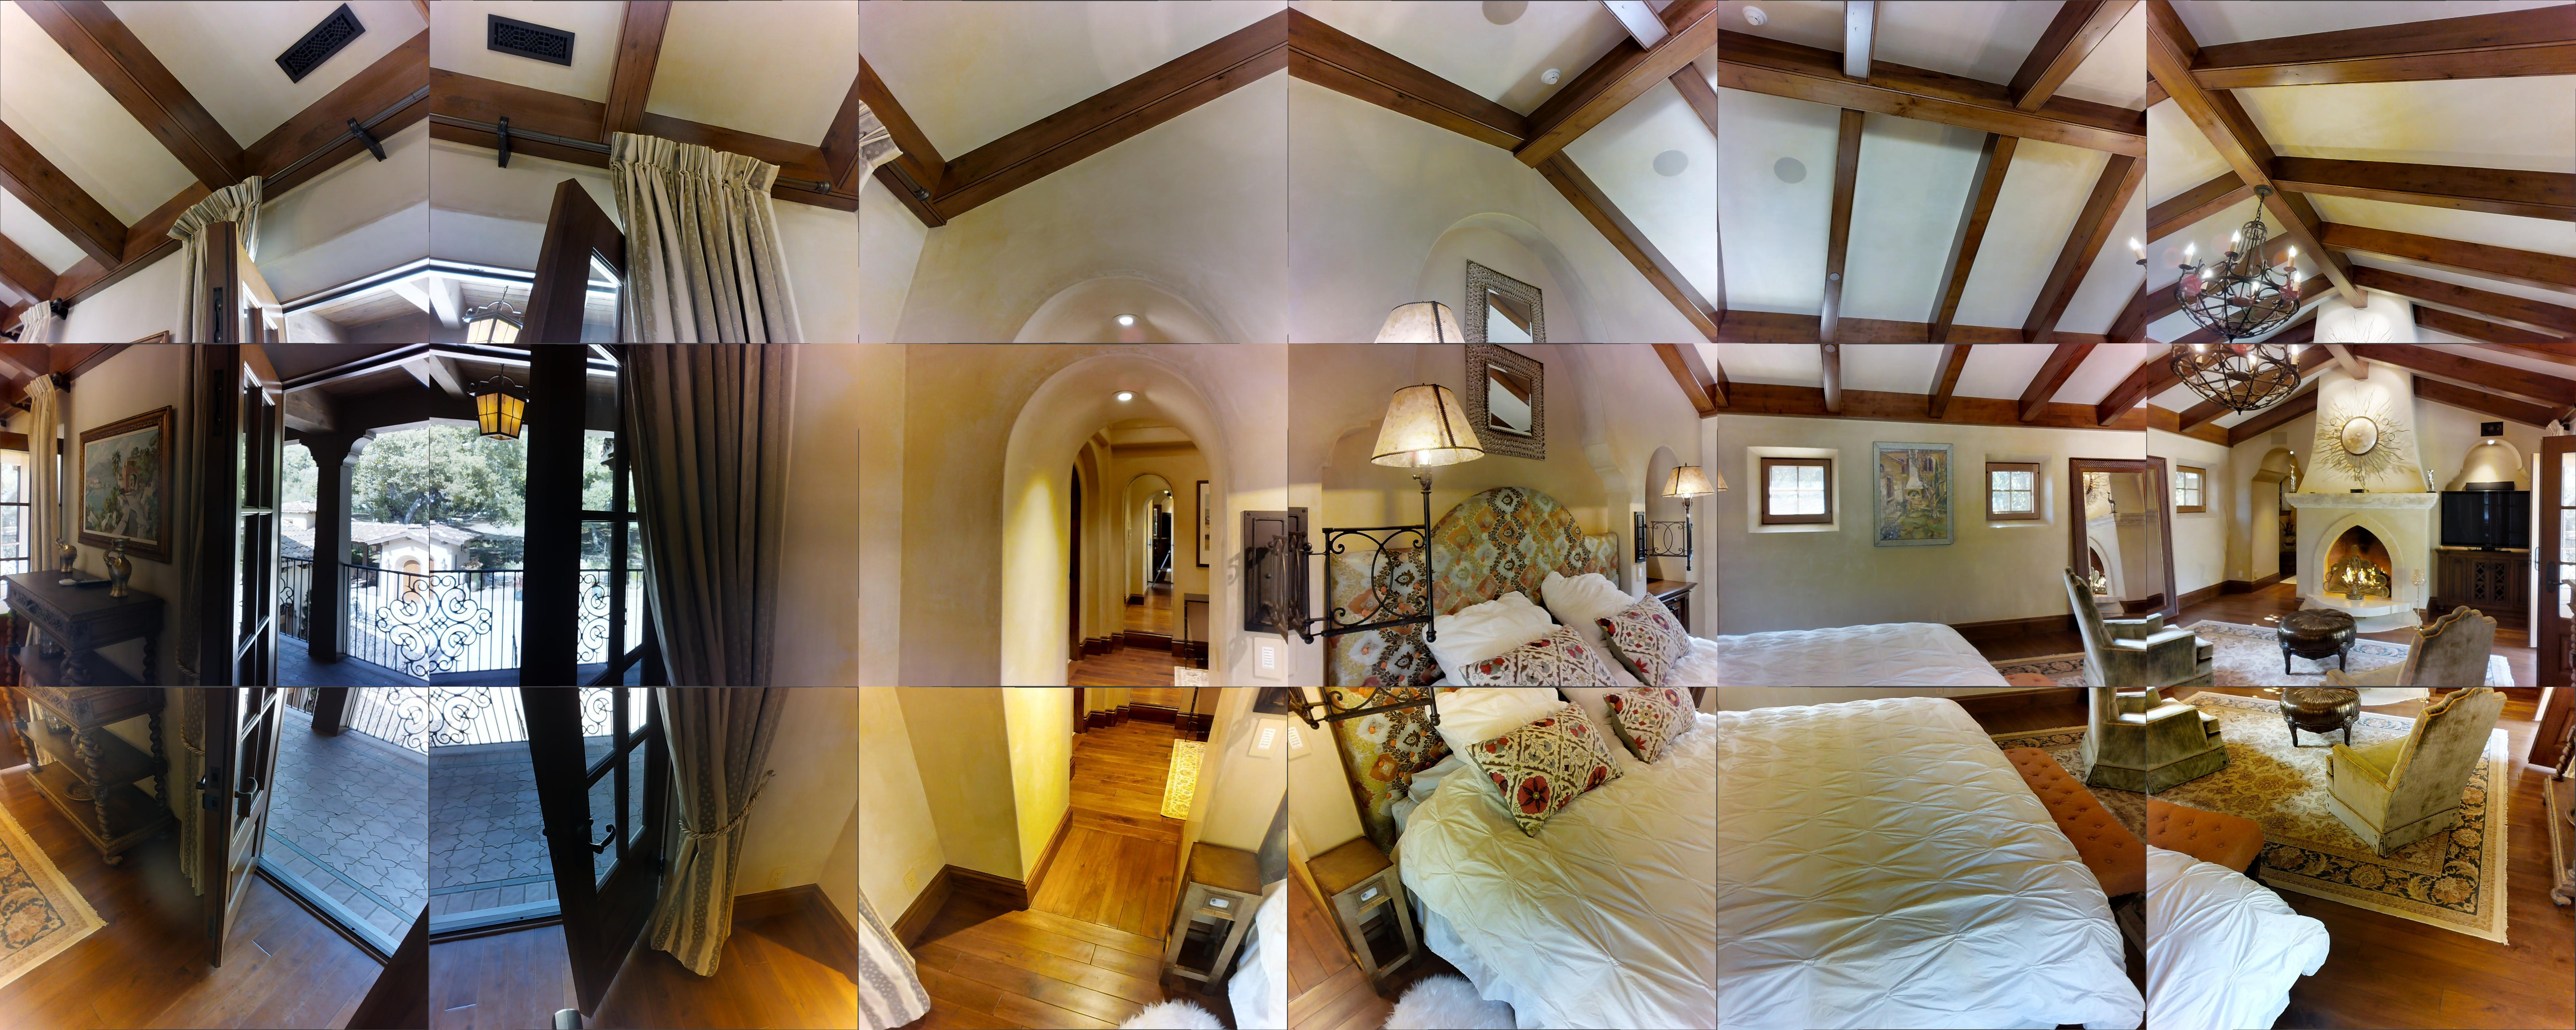
\includegraphics[width=0.8\linewidth]{figures/3-2_white_bed.jpg}
	\caption{ラベリング対象画像}
	\label{fig:white_bed}
\end{figure}

\begin{figure}[H]
	\centering
	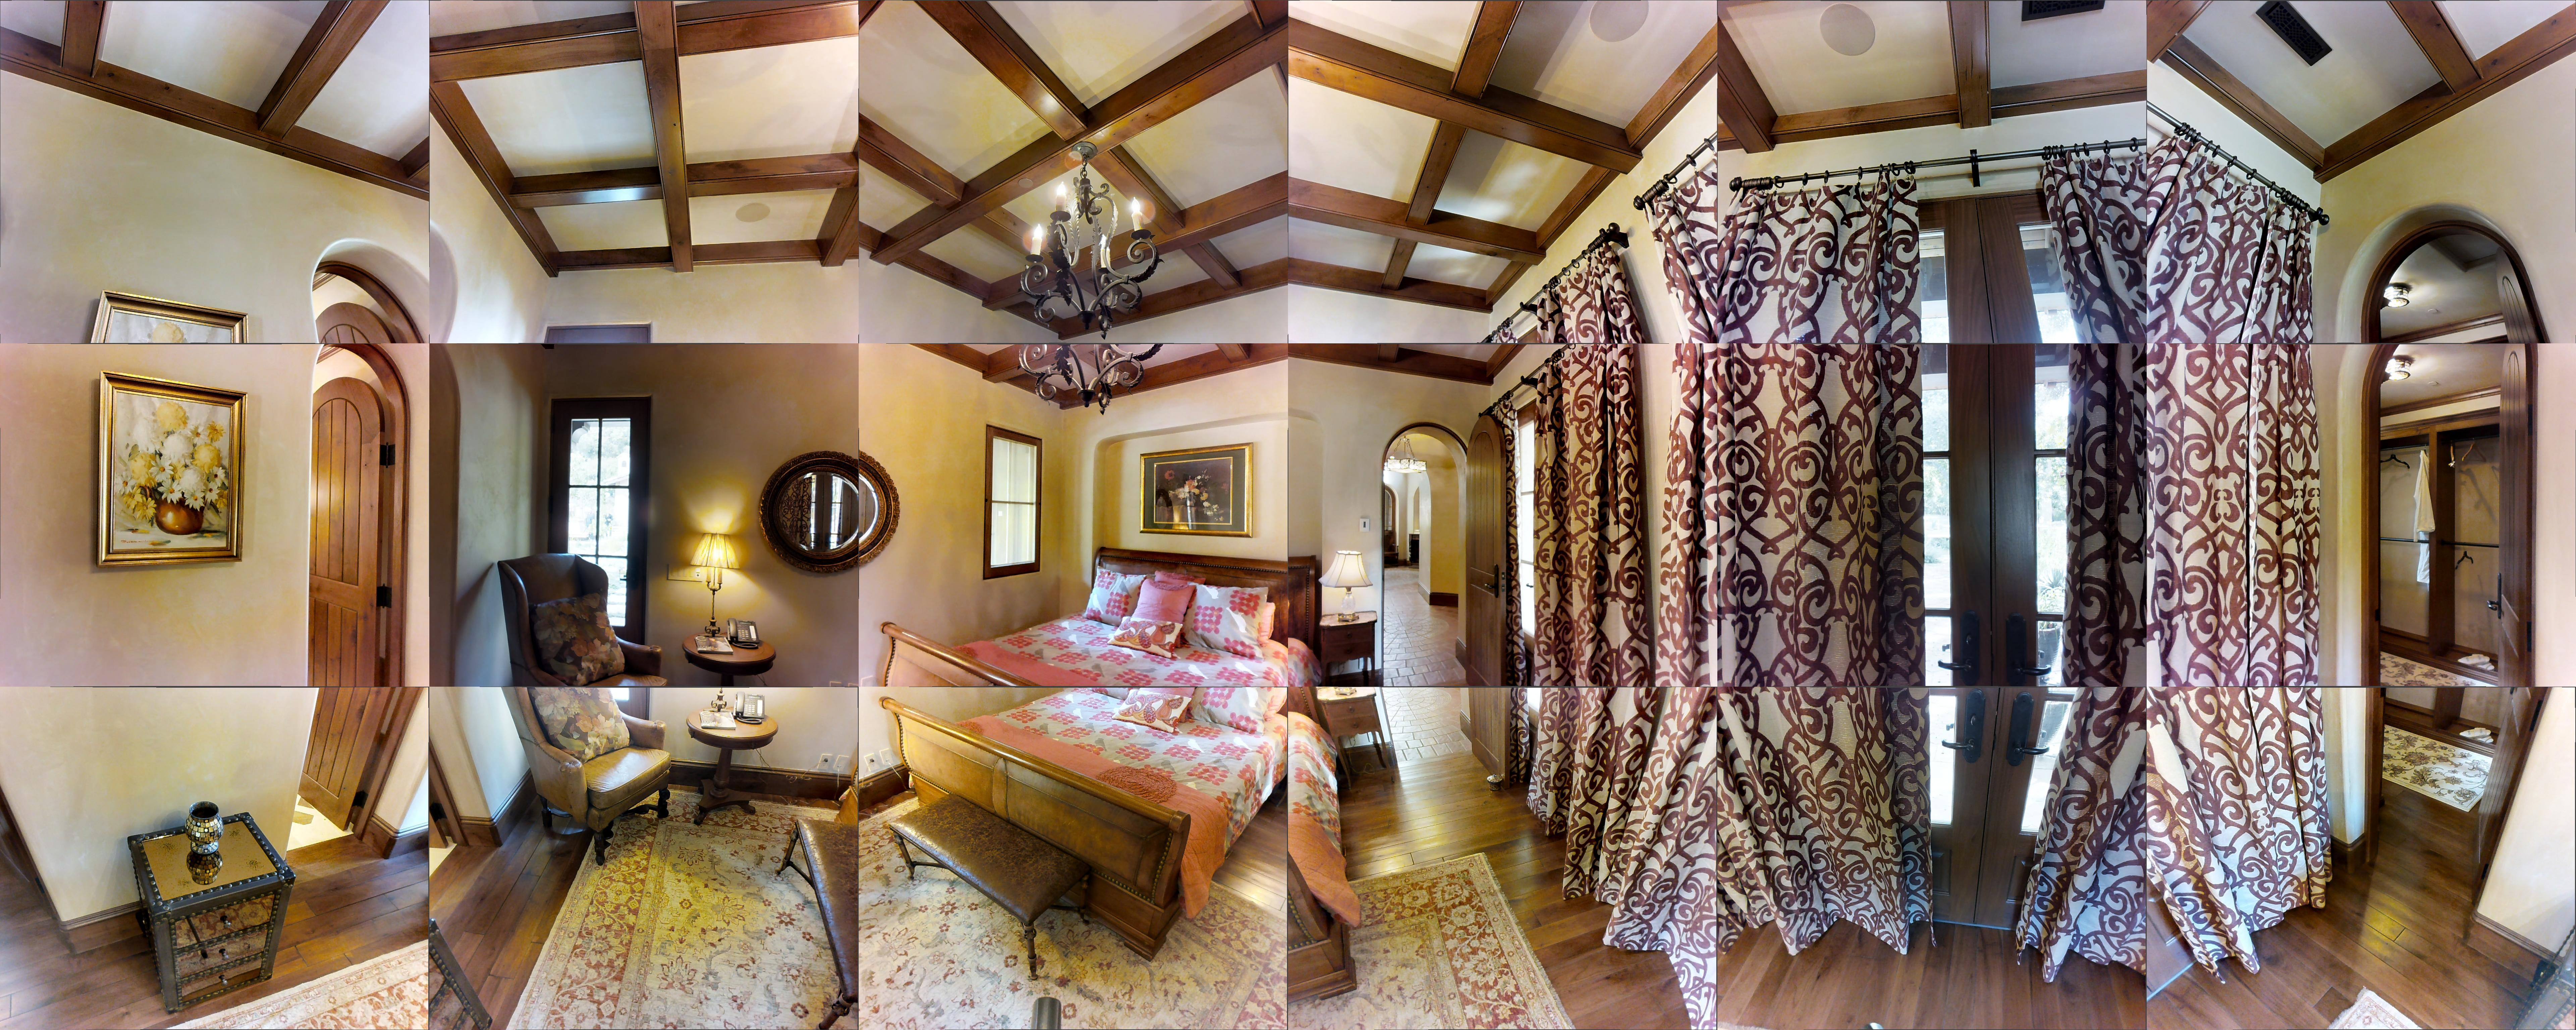
\includegraphics[width=0.8\linewidth]{figures/3-2_pink_bed.jpg}
	\caption{識別対象画像}
	\label{fig:pink_bed}
\end{figure}

この問題における,顕著性と識別性の有無を反映したラベルを,それぞれ以下に示す.

\paragraph*{顕著性と識別性どちらも低いラベル}
「広い部屋」.ラベリング対象画像の特徴を十分に説明できておらず,かつ識別対象画像との区別もできていない.
\paragraph*{顕著性が高く,識別性が低いラベル}
「天井に張り巡らされた木製の梁と,天井から吊るされたシャンデリアが特徴的な,白い壁の寝室」.
ラベリング対象画像の説明は十分できているが,識別対象画像にも同様の特徴が含まれており,2画像の区別ができていない.
\paragraph*{顕著性が低く,識別性が高いラベル}
「暖炉のある部屋」.ラベリング対象画像のみに存在する特徴「暖炉」を表現することで,識別対象画像との区別に関してはできている.
しかし,ラベリング対象画像に含まれる特徴の中で特徴「暖炉」が画像を占める面積は小さく,
画像の特徴を十分に説明できているとは言えない.
\paragraph*{顕著性と識別性どちらも高いラベル}
「木製の梁とシャンデリアが特徴的な,真っ白なベッドのある寝室」.
部屋の特長を十分に説明しており,かつ識別対象画像との区別ができる特徴「真っ白なベッド」を含んでいる.

\section{話し手モデルと聞き手モデル}

本研究では,語用論に基づくアプローチを用いて,ラベルの品質を改善する.
語用論は,言語交渉の過程において話し手と聞き手の意図の相互理解を探求する学問分野であり,
特に皮肉表現や比喩表現などの複雑な言語現象を研究対象としている.
本研究における語用論的アプローチは,話し手モデルと聞き手モデルの2つの対話モデルに基づいて構築される.
話し手モデルと聞き手モデルの双方向の対話を通じて,誤解のないラベルの生成を目指す.

話し手モデルの目的は,画像を正確に表現したラベルの生成である.
このモデルでは,画像の主要な特徴を十分に説明し,ラベルの曖昧性を排除することを重視する.

一方,聞き手モデルは,話し手モデルによって生成されたラベルが
誤解を招く可能性があるかを評価する.
このモデルはラベルが提供する情報に関して,
他のラベルとの間で起こり得る誤解の有無を検証し,
その結果を話し手モデルに対してフィードバックする.

% \section{ベースライン(ChatGPT手法)}
% プロンプトの説明中心
\section{Pragmatic ChatGPT(PCG)手法}
本研究では,前節における話し手モデルと聞き手モデルの両方にChatGPTを導入した,
Pragmatic ChatGPT(PCG)を提案する.

PCGの目的は,ラベルの識別性を高めることである.
PCGでは,話し手モデルによるラベルの生成と,聞き手モデルによるラベルの評価を行い,
この2つのモデルの処理の反復により,ラベルの誤解可能性を段階的に減少させる.

PCGにおけるラベル改善処理のプロセスを図\ref{fig:PCGflow}に示す.
ラベル改善処理では,初めに,話し手モデル1が対象画像に対する初期ラベルを生成する.
続いて,この初期ラベルに対し,聞き手モデルが改善に向けた具体的なヒントを提供する.
これらのヒントを基に,話し手モデル2は改良されたラベルを作成し,
それを再び聞き手モデルへと提出する.
このプロセスの繰り返しにより,ラベルの誤解可能性を徐々に低減させ,
ラベルの識別性を向上させることを目指す.
各サイクルは,ラベルの精度と明確性の向上に寄与し,
最終的にはより効果的な画像認識と解釈を可能にすることが期待される.

\begin{figure}[H]
	\centering
	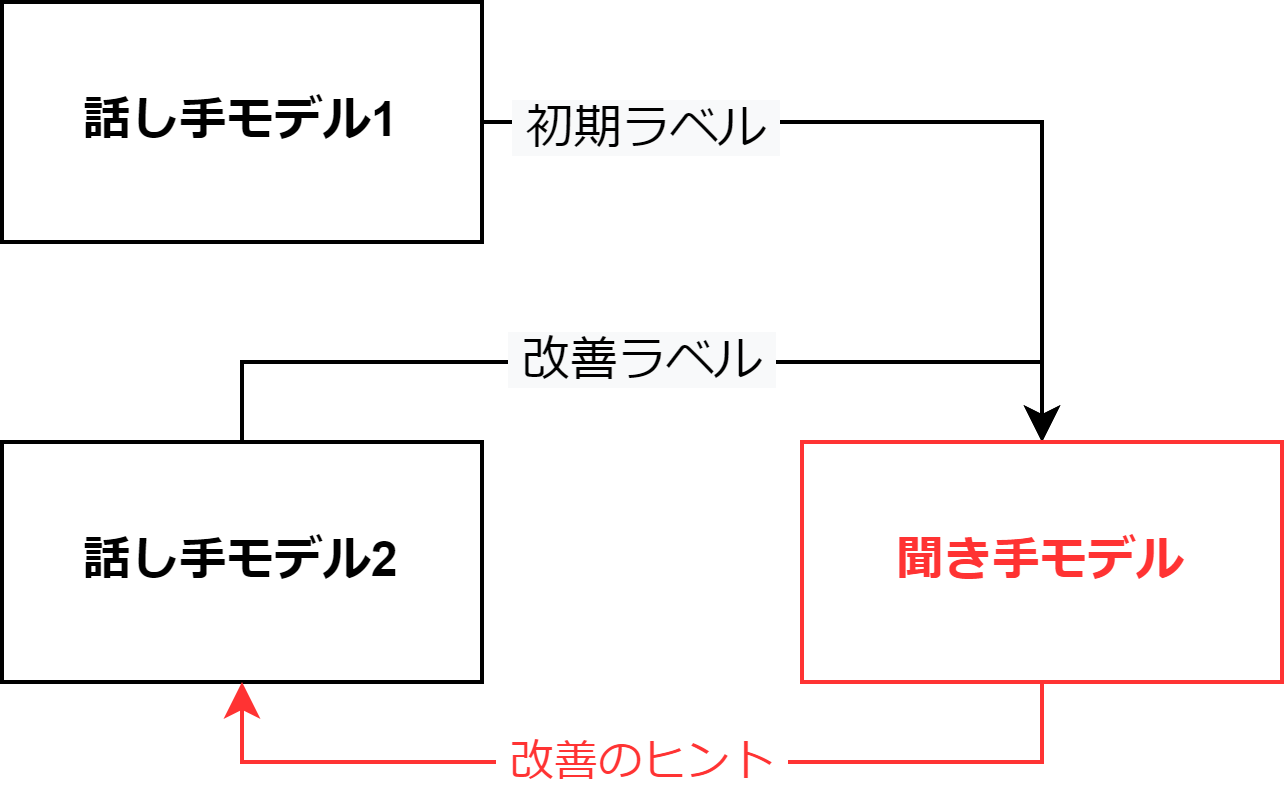
\includegraphics[width=0.8\linewidth]{figures/PCGflow.png}
	\caption{ラベル改善フロー}
	\label{fig:PCGflow}
\end{figure}

図\ref{fig:PCGflow}における,話し手モデル1(初期ラベル生成フロー)の処理の流れを図\ref{fig:PCGspeaker1}に示す.
話し手モデル1は,入力された画像の集合に対して,各画像の特徴を説明するようなキャプション生成を行う.
このとき,話し手モデル2にあるような,ラベル改善のヒントを踏まえた生成などは行わず,
純粋なキャプショニングによってラベルを生成する.

\begin{figure}[H]
	\centering
	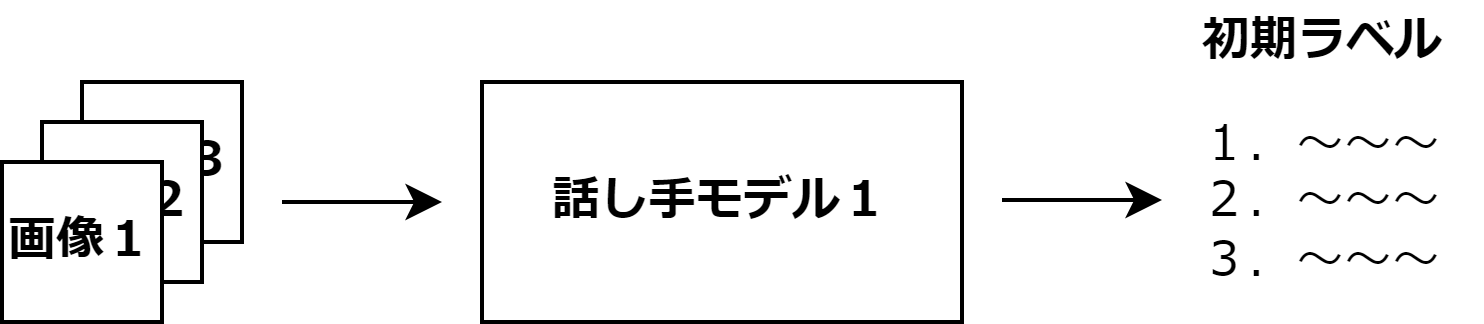
\includegraphics[width=0.8\linewidth]{figures/PCGspeaker1.png}
	\caption{話し手モデル1(初期ラベル生成フロー)}
	\label{fig:PCGspeaker1}
\end{figure}

次に図\ref{fig:PCGflow}における聞き手モデル(ヒント生成フロー)の処理の流れを図\ref{fig:PCGlistener}に示す.
聞き手モデルは,入力された画像の集合と,話し手モデルによって生成されたラベルから,
各ラベルの誤解可能性について評価を行い,ラベルの改善に役立つヒントを出力する.

\begin{figure}[H]
	\centering
	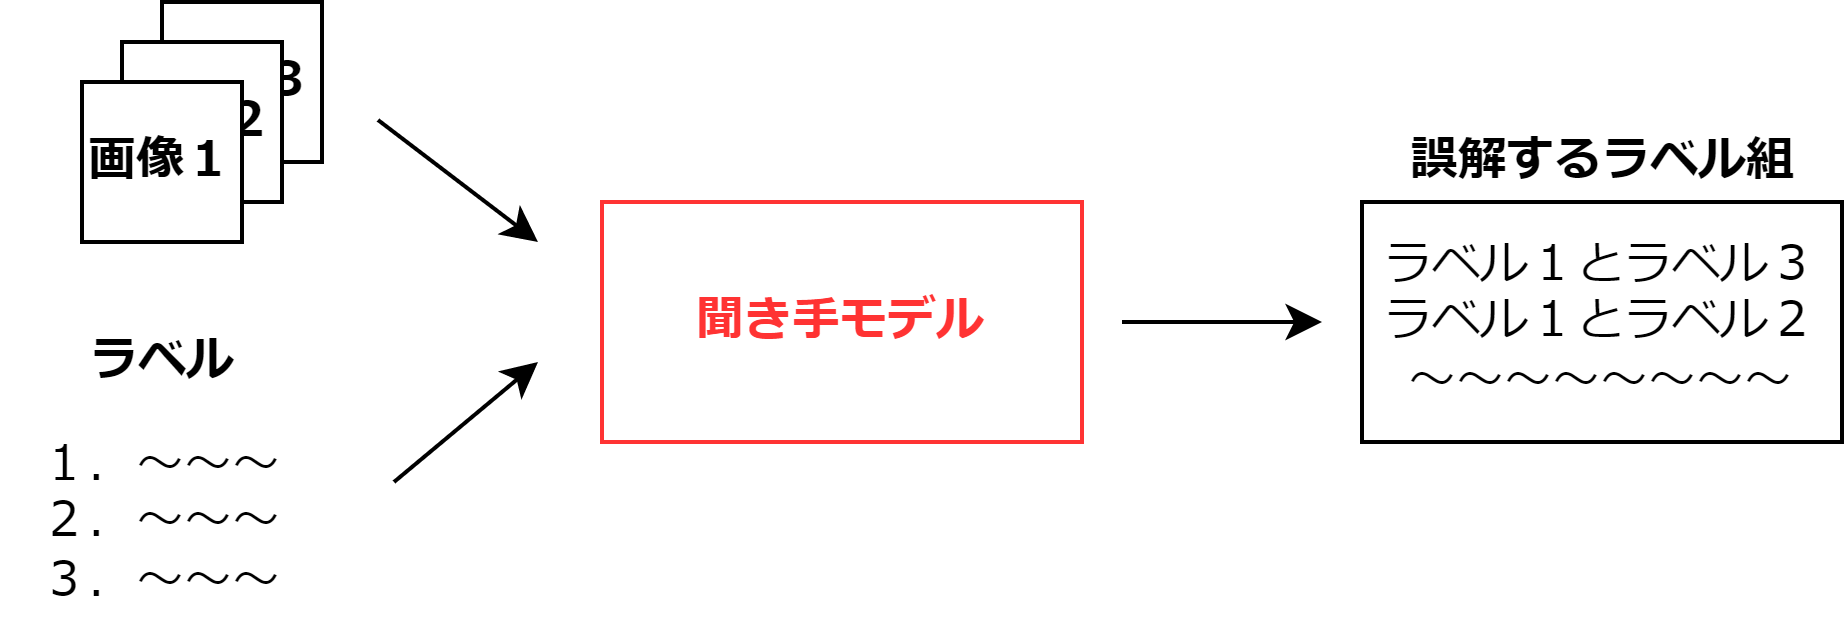
\includegraphics[width=0.8\linewidth]{figures/PCGlistener.png}
	\caption{聞き手モデル(ヒント生成フロー)}
	\label{fig:PCGlistener}
\end{figure}

聞き手モデルが生成するヒントは,誤解する可能性の高い2つのラベルの組み合わせを示す形式をとる.
例えば,ラベル1とラベル3に同じ単語が含まれており,
それぞれのラベルに対応する画像にも同様の特徴が含まれていた場合,
そのラベル組の識別性は互いに低くなると考えられる.
そのような場合,そのラベルの組の誤解可能性が高いとして,
改善すべきラベル組はラベル1とラベル3である,といったようにラベル改善のヒントを出力する.

具体的には以下の形式で出力を行う.
\begin{eqnarray}
  ラベルAとラベルB:(ラベルAとラベルB間で誤解可能性が高くなる要因)  
\end{eqnarray}

実際に出力されるヒントの例を図\ref{fig:hint_example}に示す.

\begin{figure}[H]
  \begin{mdframed}[linewidth=1pt]
    hint 1. Caption 3 and Caption 10: Both mention contemporary elements with large windows and a spacious layout, which could refer to modern architecture with a minimalist theme.
  \end{mdframed}
  \caption{出力されるラベル改善のヒントの例}
  \label{fig:hint_example}
\end{figure}

最後に図\ref{fig:PCGflow}における話し手モデル2(ラベル改善フロー)の処理の流れを図\ref{fig:PCGspeaker2}に示す.
話し手モデル2では,画像の集合,既に生成されているラベル,聞き手モデルによって生成されたラベル改善のヒントをもとに,
新たなラベルを生成する.
このとき,ラベル改善のヒントをもとにして既に生成されているラベルの改善を行うことで,
よりラベルの誤解可能性を小さくすることを狙う.

\begin{figure}[H]
	\centering
	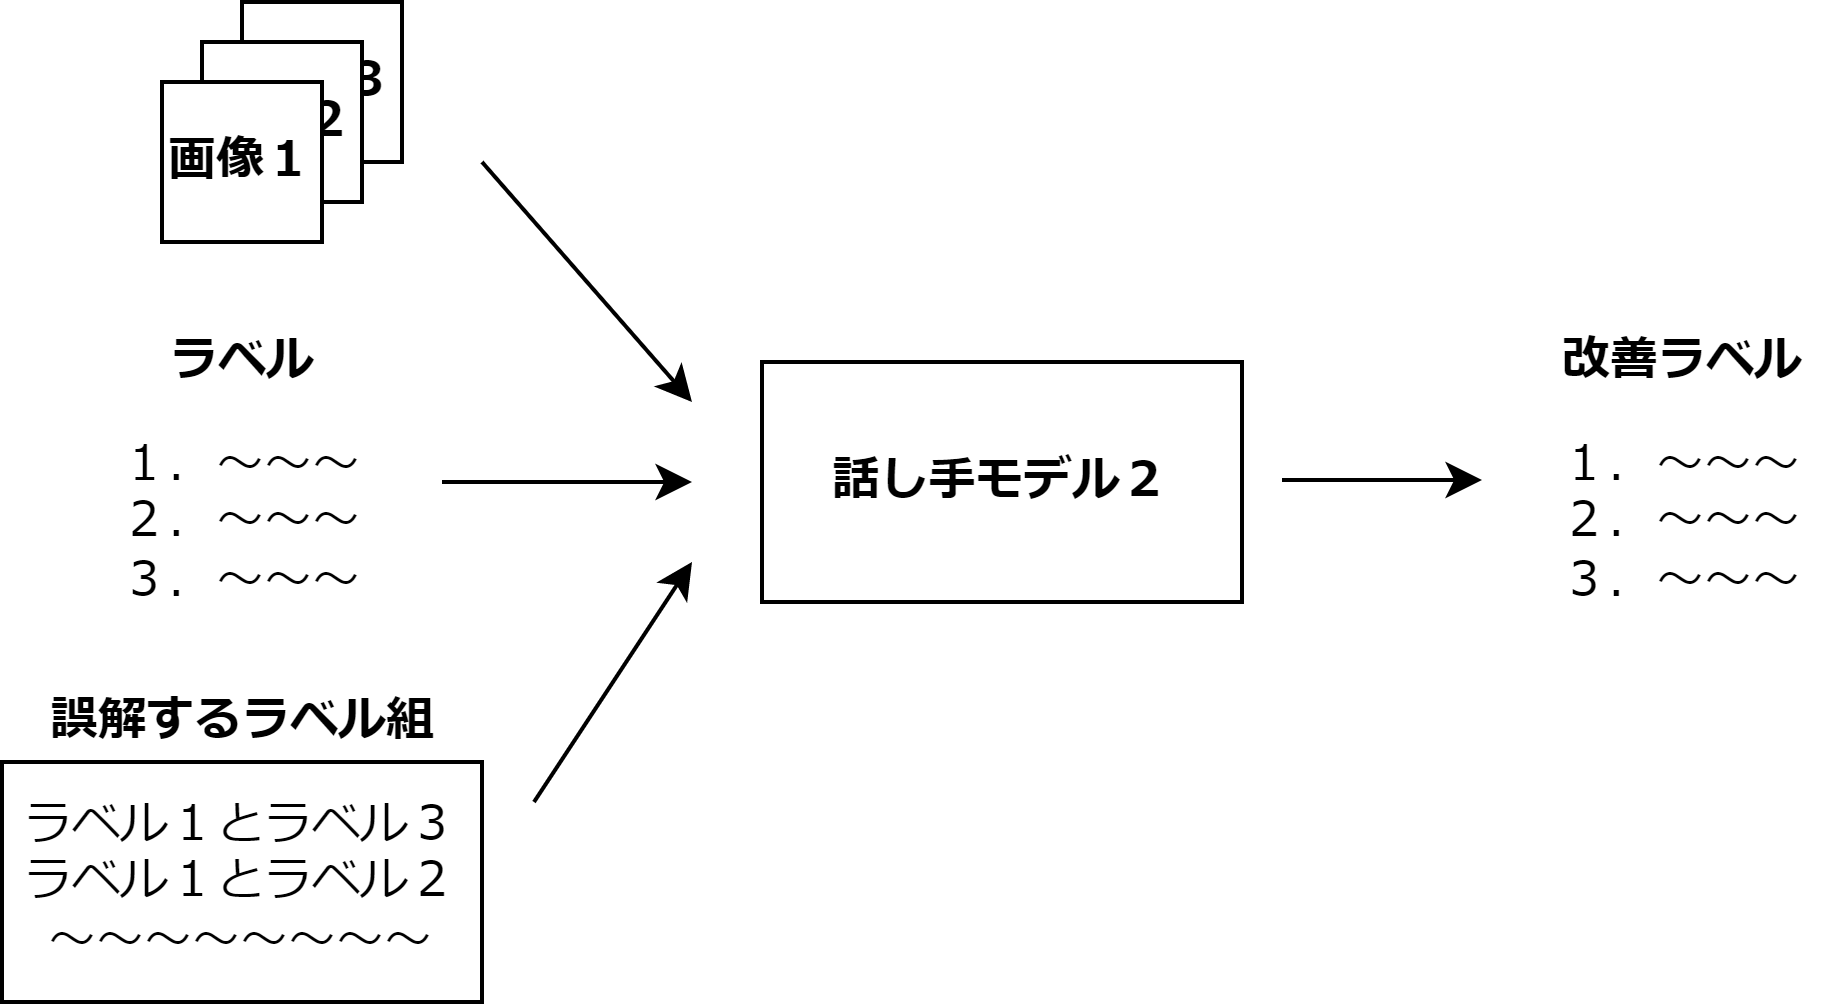
\includegraphics[width=0.8\linewidth]{figures/PCGspeaker2.png}
	\caption{話し手モデル2(ラベル改善フロー)}
	\label{fig:PCGspeaker2}
\end{figure}

画像の集合をX,n回目の改善サイクルにおけるラベルをYn,n回目の改善サイクルにおけるヒントをH,
改善サイクルを回す回数をmとして,
ここまでのラベル改善処理をまとめた流れは以下の通りである.

\begin{enumerate}
  \item ChatGPTに対して画像の集合Xを入力する.Xに含まれる各画像に対して,それぞれ誤解なく画像を区別できるラベルを出力するように,プロンプトを入力する.ここで出力されたラベルの集合をY1とする.
  \item ラベルの集合Y1と画像の集合XをChatGPTに入力する.Y1に含まれる各ラベルについて誤解可能性を分析し,ラベル改善のヒントを出力するように,プロンプトを入力する.出力されたラベル改善のヒントをH1とする.
  \item ChatGPTに対して画像の集合X,ラベル改善のヒントH1,ラベルの集合Y1を入力する.H1を参考にして,Y1を改善した新たなラベルを出力するように,プロンプトを入力する.ここで出力されたラベルの集合をY2とする.
  \item 2と3を繰り返して,最終的に得られたラベルの集合Ym(mは任意の自然数)を,誤解可能性の低いラベルとして提出する.
\end{enumerate}


% 実験
\chapter{評価実験}

\section{実験設定}

本実験では,各手法の性能を比較するため,生成されたラベルの誤解可能性を検証する.被験者に複数の画像と1つのラベルを与え,対応する画像を選択できるかを調査する.

実験全体の流れをまとめた図を図\ref{fig:flow_example}に示す.図の左部は手法によるラベルの評価部分で,右部は被験者実験によるラベルの評価部分である.

\begin{figure}[H]
  \centering
  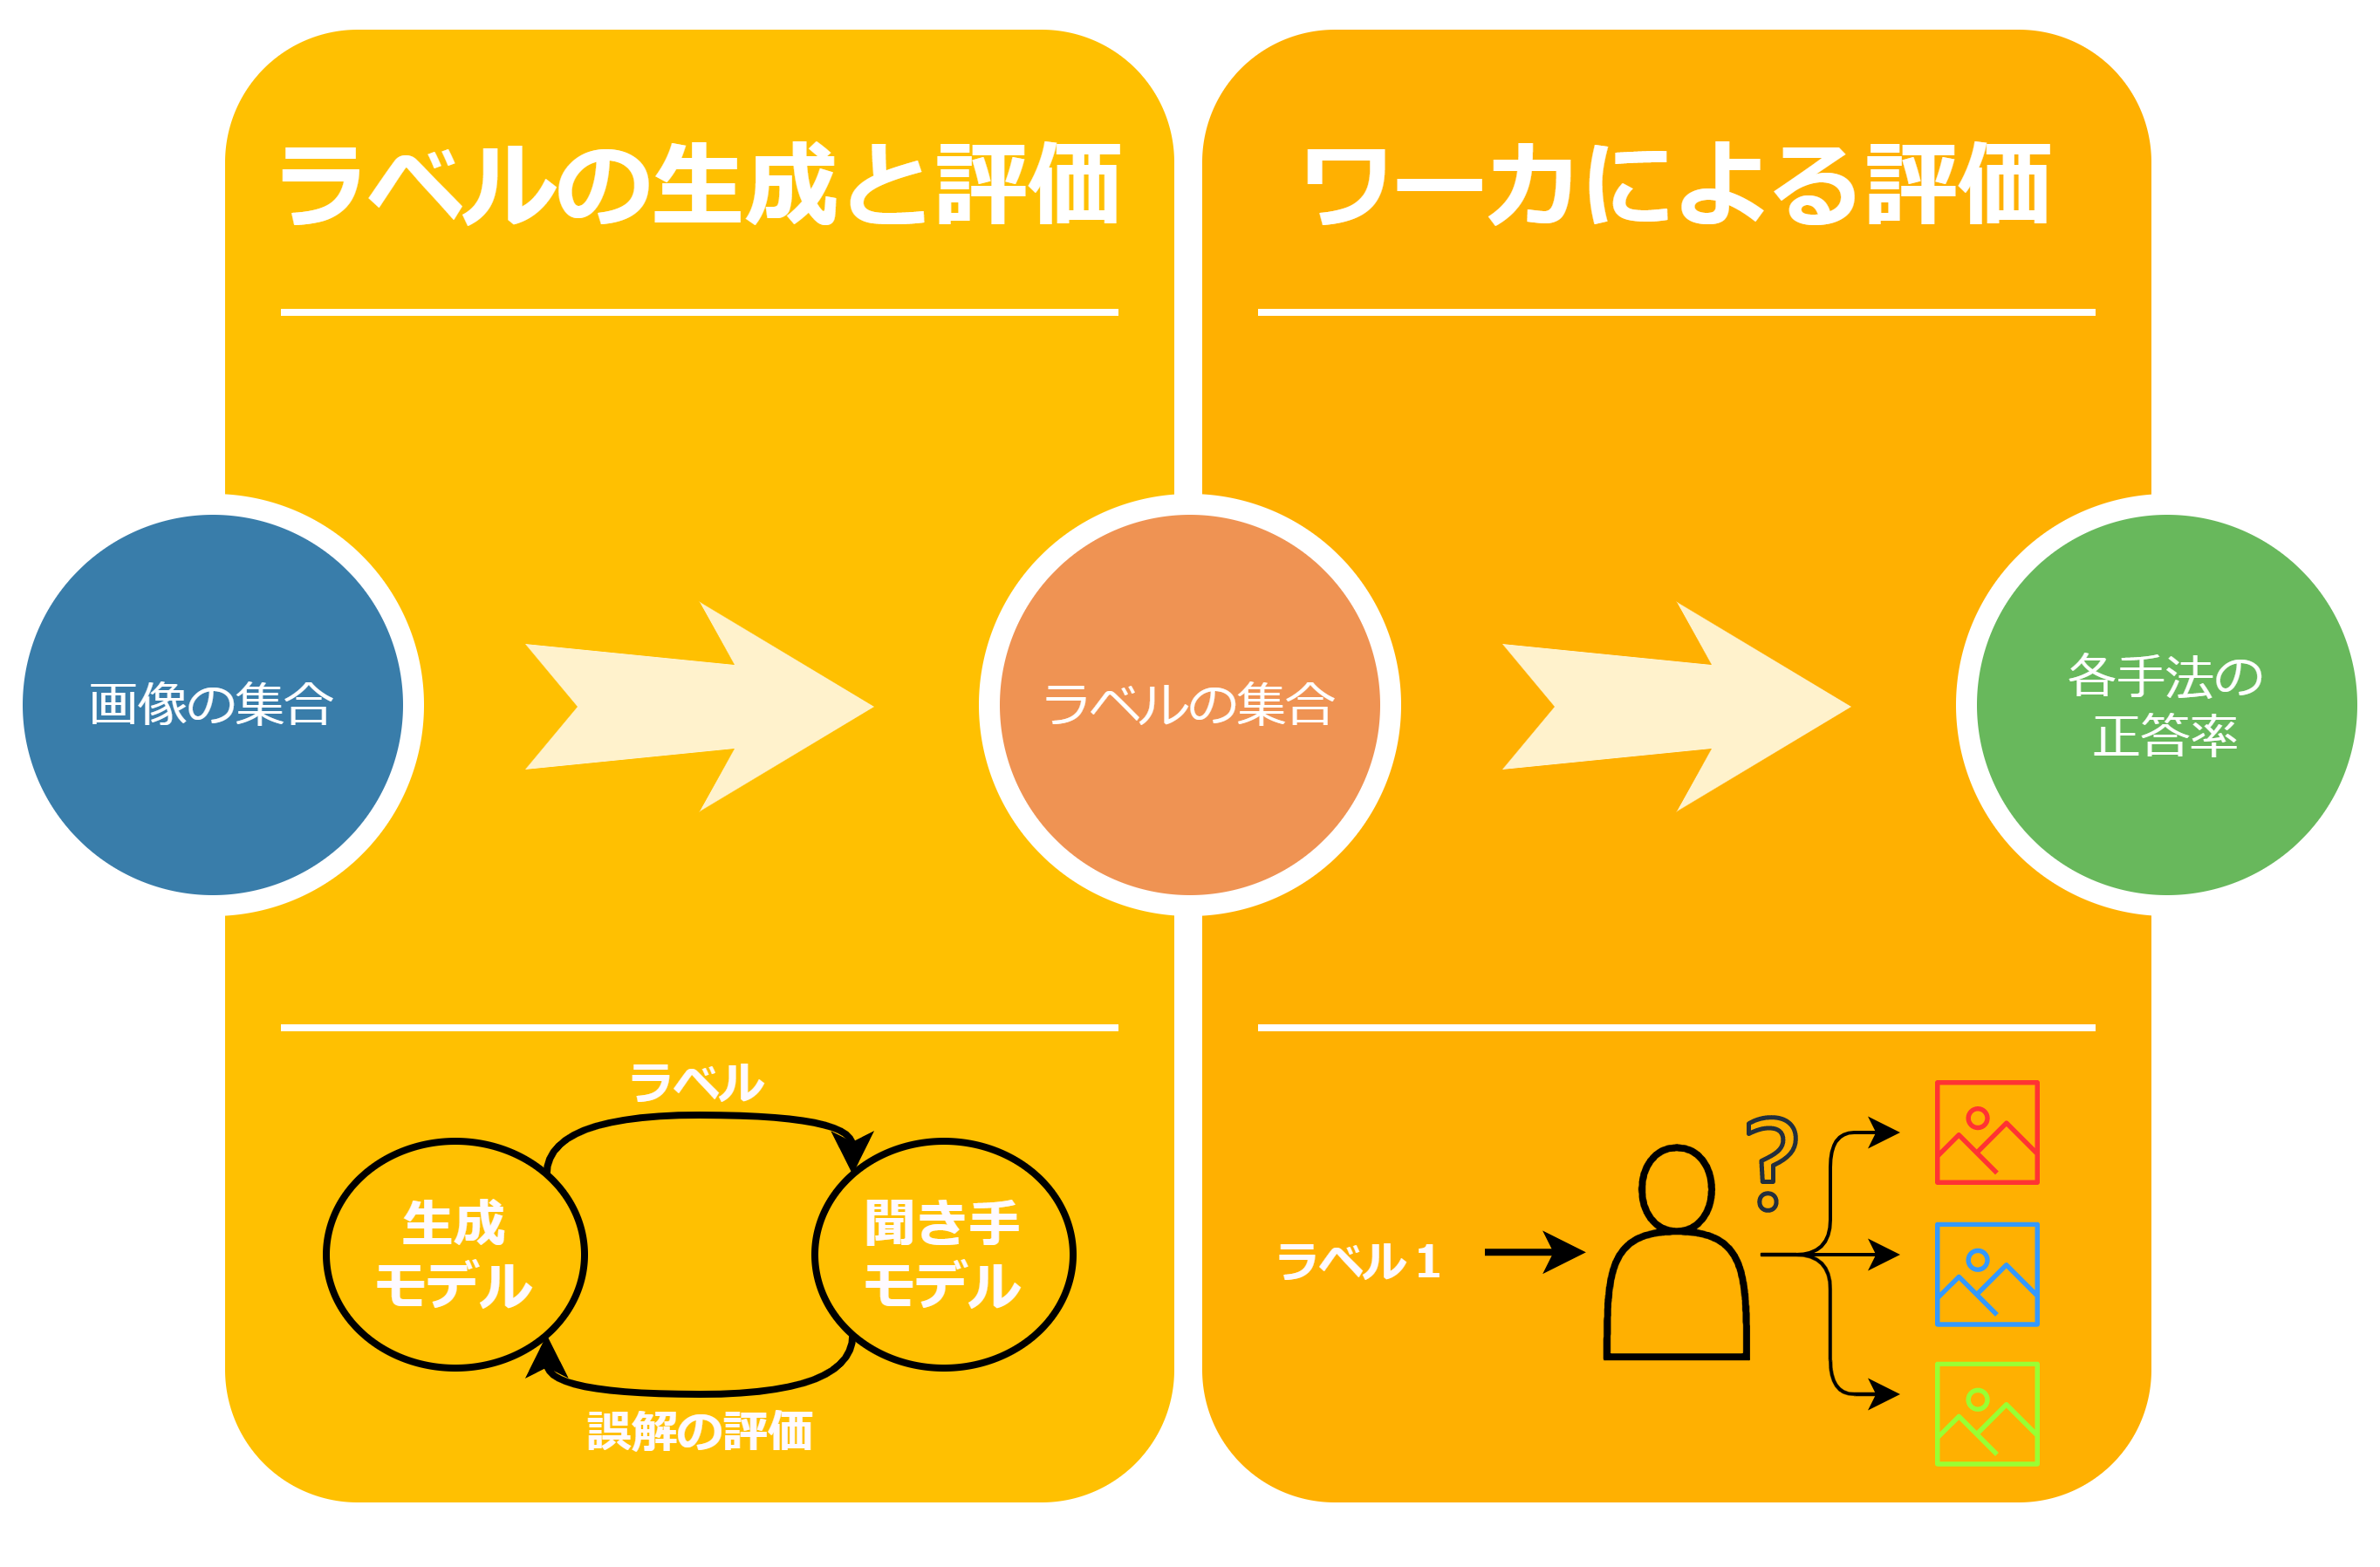
\includegraphics[width=\linewidth]{figures/flow.png}
  \caption{実験の流れ}
  \label{fig:flow_example}
\end{figure}


ラベルの生成には以下の2つの手法を用いる.
\begin{enumerate}
    \item ChatGPTを用いたベースライン手法
    \item Pragmatic ChatGPT
\end{enumerate}

ChatGPTを用いたベースライン手法は,ChatGPTを用いて画像に対して1対1でラベルを生成する単純な手法である.ChatGPTを用いたベースライン手法を評価基準とし,これとの比較により提案手法の評価を行う.ベースライン手法の詳細な処理内容は4.2節で述べる.

また,実用性と汎用性の評価のために,それぞれの手法でラベル長を制限することによる以下の2種類の出力方法でラベル生成を行い,被験者実験による手法の評価に用いる.

\begin{enumerate}
    \item 通常出力(normal output):ラベル長に制限を設けずに出力
    \item 短出力(minimal output):ラベル長を制限(例:10単語以内)して出力
\end{enumerate}

ラベルの生成元となる画像には,Matterport3Dデータセットを使用する.データセット内に含まれる,同一地点から撮影した部屋の画像を結合することによってパノラマ画像を得る.パノラマ画像を1つの部屋を表す概念として扱い,いくつかの部屋のパノラマ画像に対してラベリングを行う.データセットの詳細は4.1.1節で述べる.

被験者実験はAmazon Mechanical Turk(AMT)を使用して行う.AMTはマイクロタスク型のクラウドソーシングサービスである.ワーカーに対してタスクをリクエストし,ワーカーがアクションを行い,その結果を回収する.

本実験では,ワーカーに複数の画像とラベルを与え,ラベルに紐づく画像を選択してもらう.AMTタスクの詳細は4.1.2節で述べる.

\subsection{データセット}

実験では,Matterport3Dデータセット\footnote{https://niessner.github.io/Matterport/}を使用する.Matterport3Dデータセットは,90の建物から成る,194,400枚のRGB-D画像による大規模なRGB-Dデータセットである.

実験では,データセットに含まれる画像に対してパノラマ画像化処理を行った後,寝室を撮影した画像10枚を抽出して実験に使用した.
パノラマ画像化処理について,詳細を述べる.
データセットは,上下と水平方向の合わせて3回,それを60度ずつ横方向にずらして6回,計18回の撮影を同一の地点で行った画像群で構成されている.実験では,同一地点で撮影した18枚の画像を適切な位置で結合する処理を,すべての画像に対して行うことで,各撮影地点ごとにパノラマ画像を作成した.

生成したパノラマ画像の例を図\ref{fig:panorama_example}に示す.

\begin{figure}[H]
  \centering
  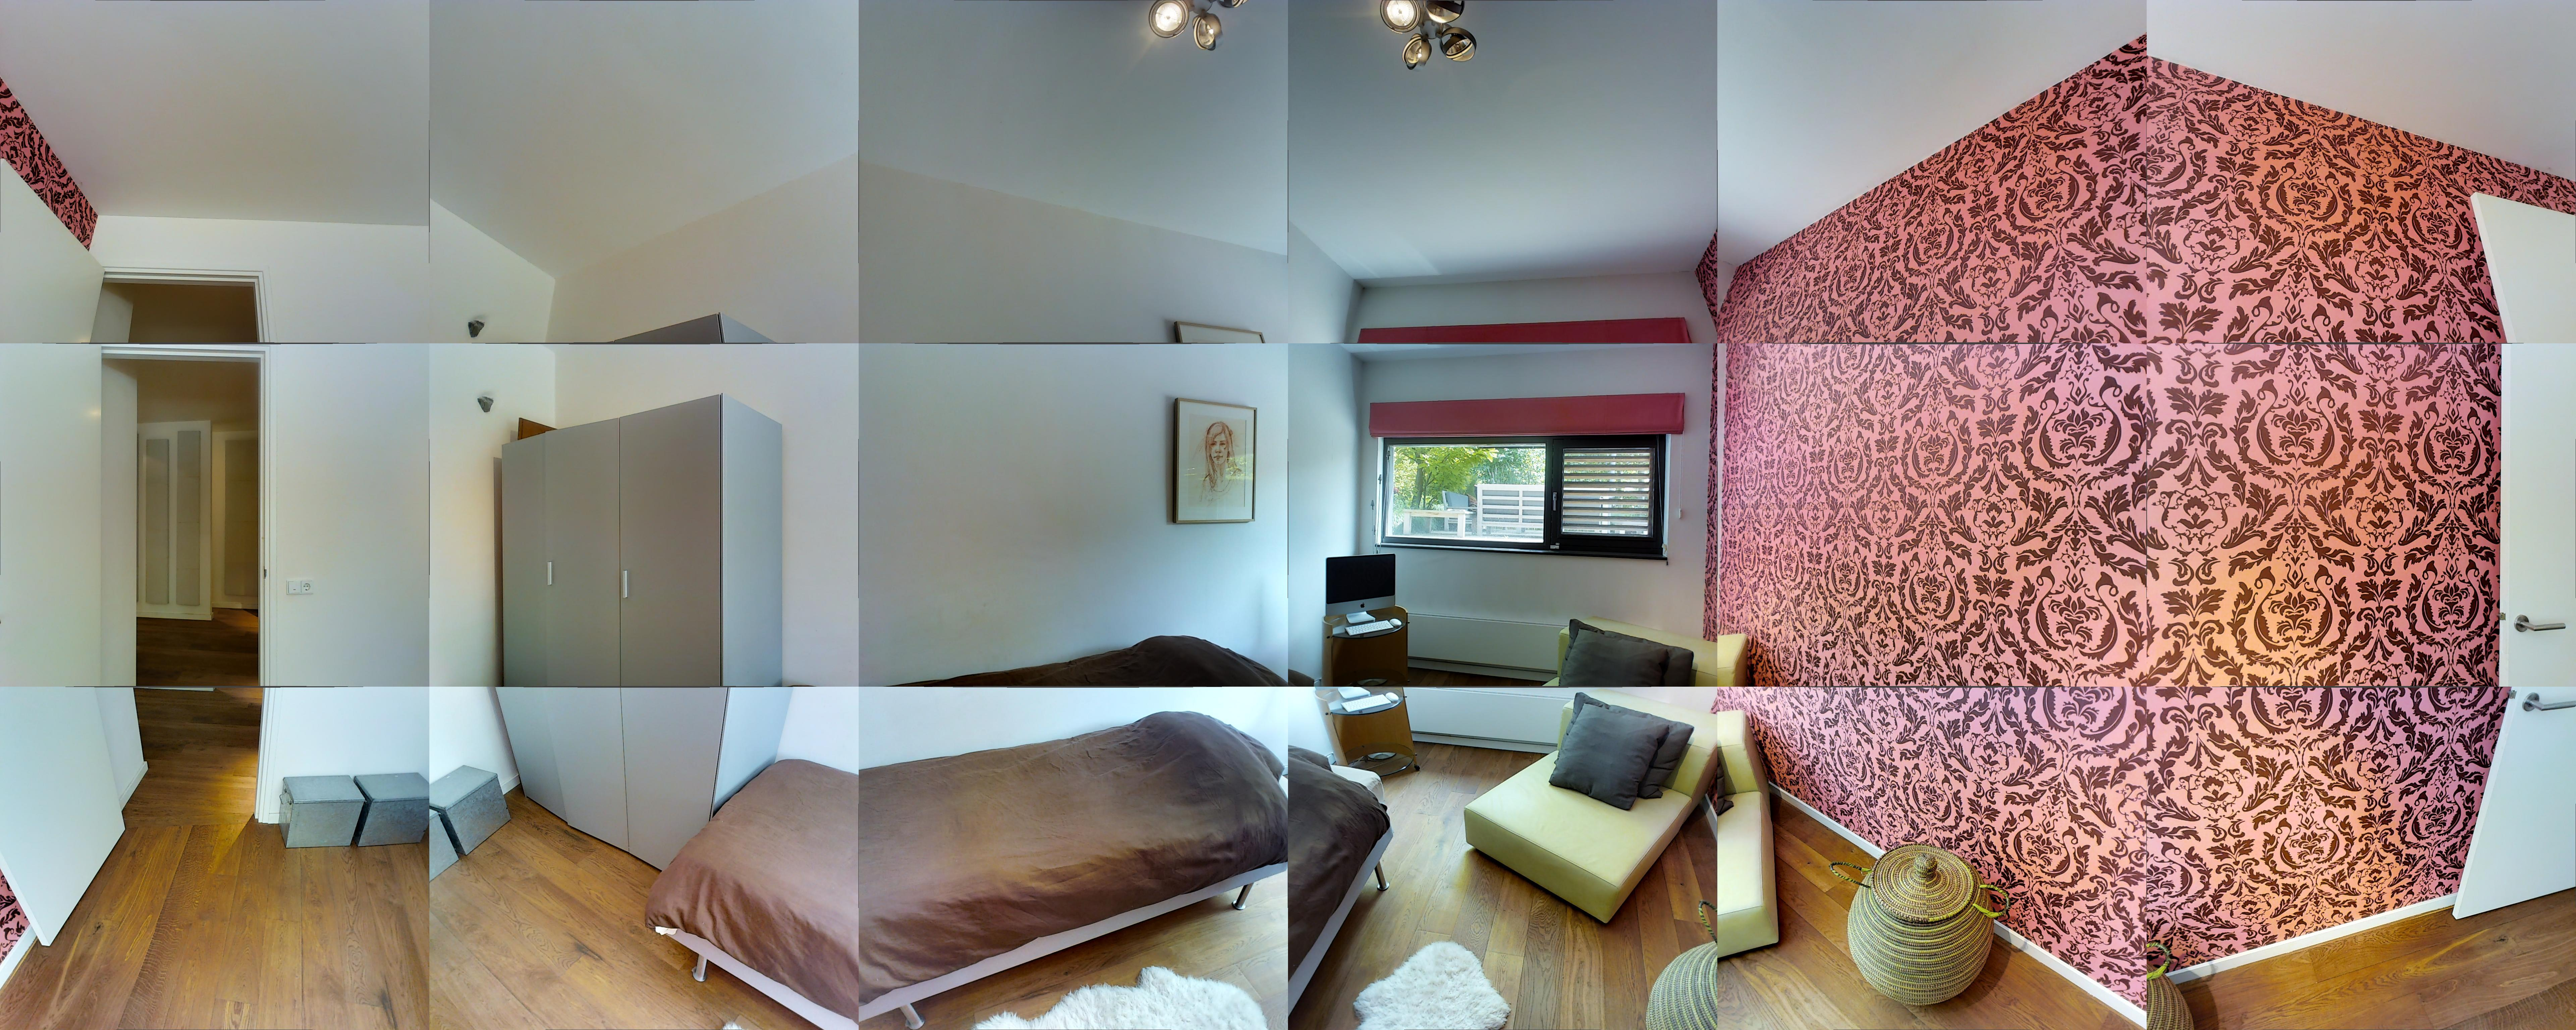
\includegraphics[width=\linewidth]{figures/panorama.jpeg}
  \caption{同一地点で撮影した画像18枚を結合したパノラマ画像}
  \label{fig:panorama_example}
\end{figure}

実験では,パノラマ画像の中から寝室を撮影した画像10枚を抽出して使用した.

\paragraph{パノラマ画像を実験で使用する理由}
ラベリング対象とする画像をパノラマ画像とする理由は,画像に含まれる特徴量を均一化するためである.データセットに含まれる画像のうち,家具や照明など部屋全体の特徴を捉えた画像はラベリングの対象として適切だが,壁のみが写っている等の部屋の特徴を含まない画像はラベリングの対象として適切ではない.このような,画像に含まれる特徴量の不均一によって引き起こされる意図的ではないラベリング精度の低下を回避するために,事前にパノラマ画像化処理を行い画像の特徴量を均一化する.

\paragraph{寝室の画像のみを抽出する理由}
ラベリング対象とする画像を寝室だけに制限する理由は,実験の難易度を適切に設定するためである.実験で使用するデータセットに含まれる画像の部屋の種類はキッチンやバスルーム,リビングなど複数存在している.これらの異なる種類の部屋の画像に対してラベリングを行った場合,「調理器具」「ベッド」などの一つ単語で各画像を容易に区別できる可能性がある.このような,画像同士の識別性を不用意に向上させかねない要因を排除するために,データセットから寝室の画像のみを抽出して実験に使用した.

\subsection{Amazon Mechanical Turk:AMTの概要}

Amazon Mechanical Turk(AMT)はマイクロタスク型に特化したクラウドソーシングサービスである.ワーカに対して何らかのタスク(アンケート,データラベリングなど)をリクエストし,ワーカがタスクに対して何らかのアクション(アンケートに回答する,データにラベルを付与するなど)を行い,ワーカが入力したデータを回収することで,問題を解決する.

実験では,4枚の画像からラベルに対応する画像を選ぶタスクを100回行い,その正答率を手法ごとに比較する.

実験で行うAMTのタスクの設定を以下に示す.

\begin{itemize}
  \item ワーカに対して4枚の画像とラベルを与える.
  \item ワーカは,ラベルに紐づくと考えられる画像を一枚選択する.
\end{itemize}

AMTタスクの例を図\ref{fig:amt_example}に示す.

\begin{figure}[H]
  \centering
  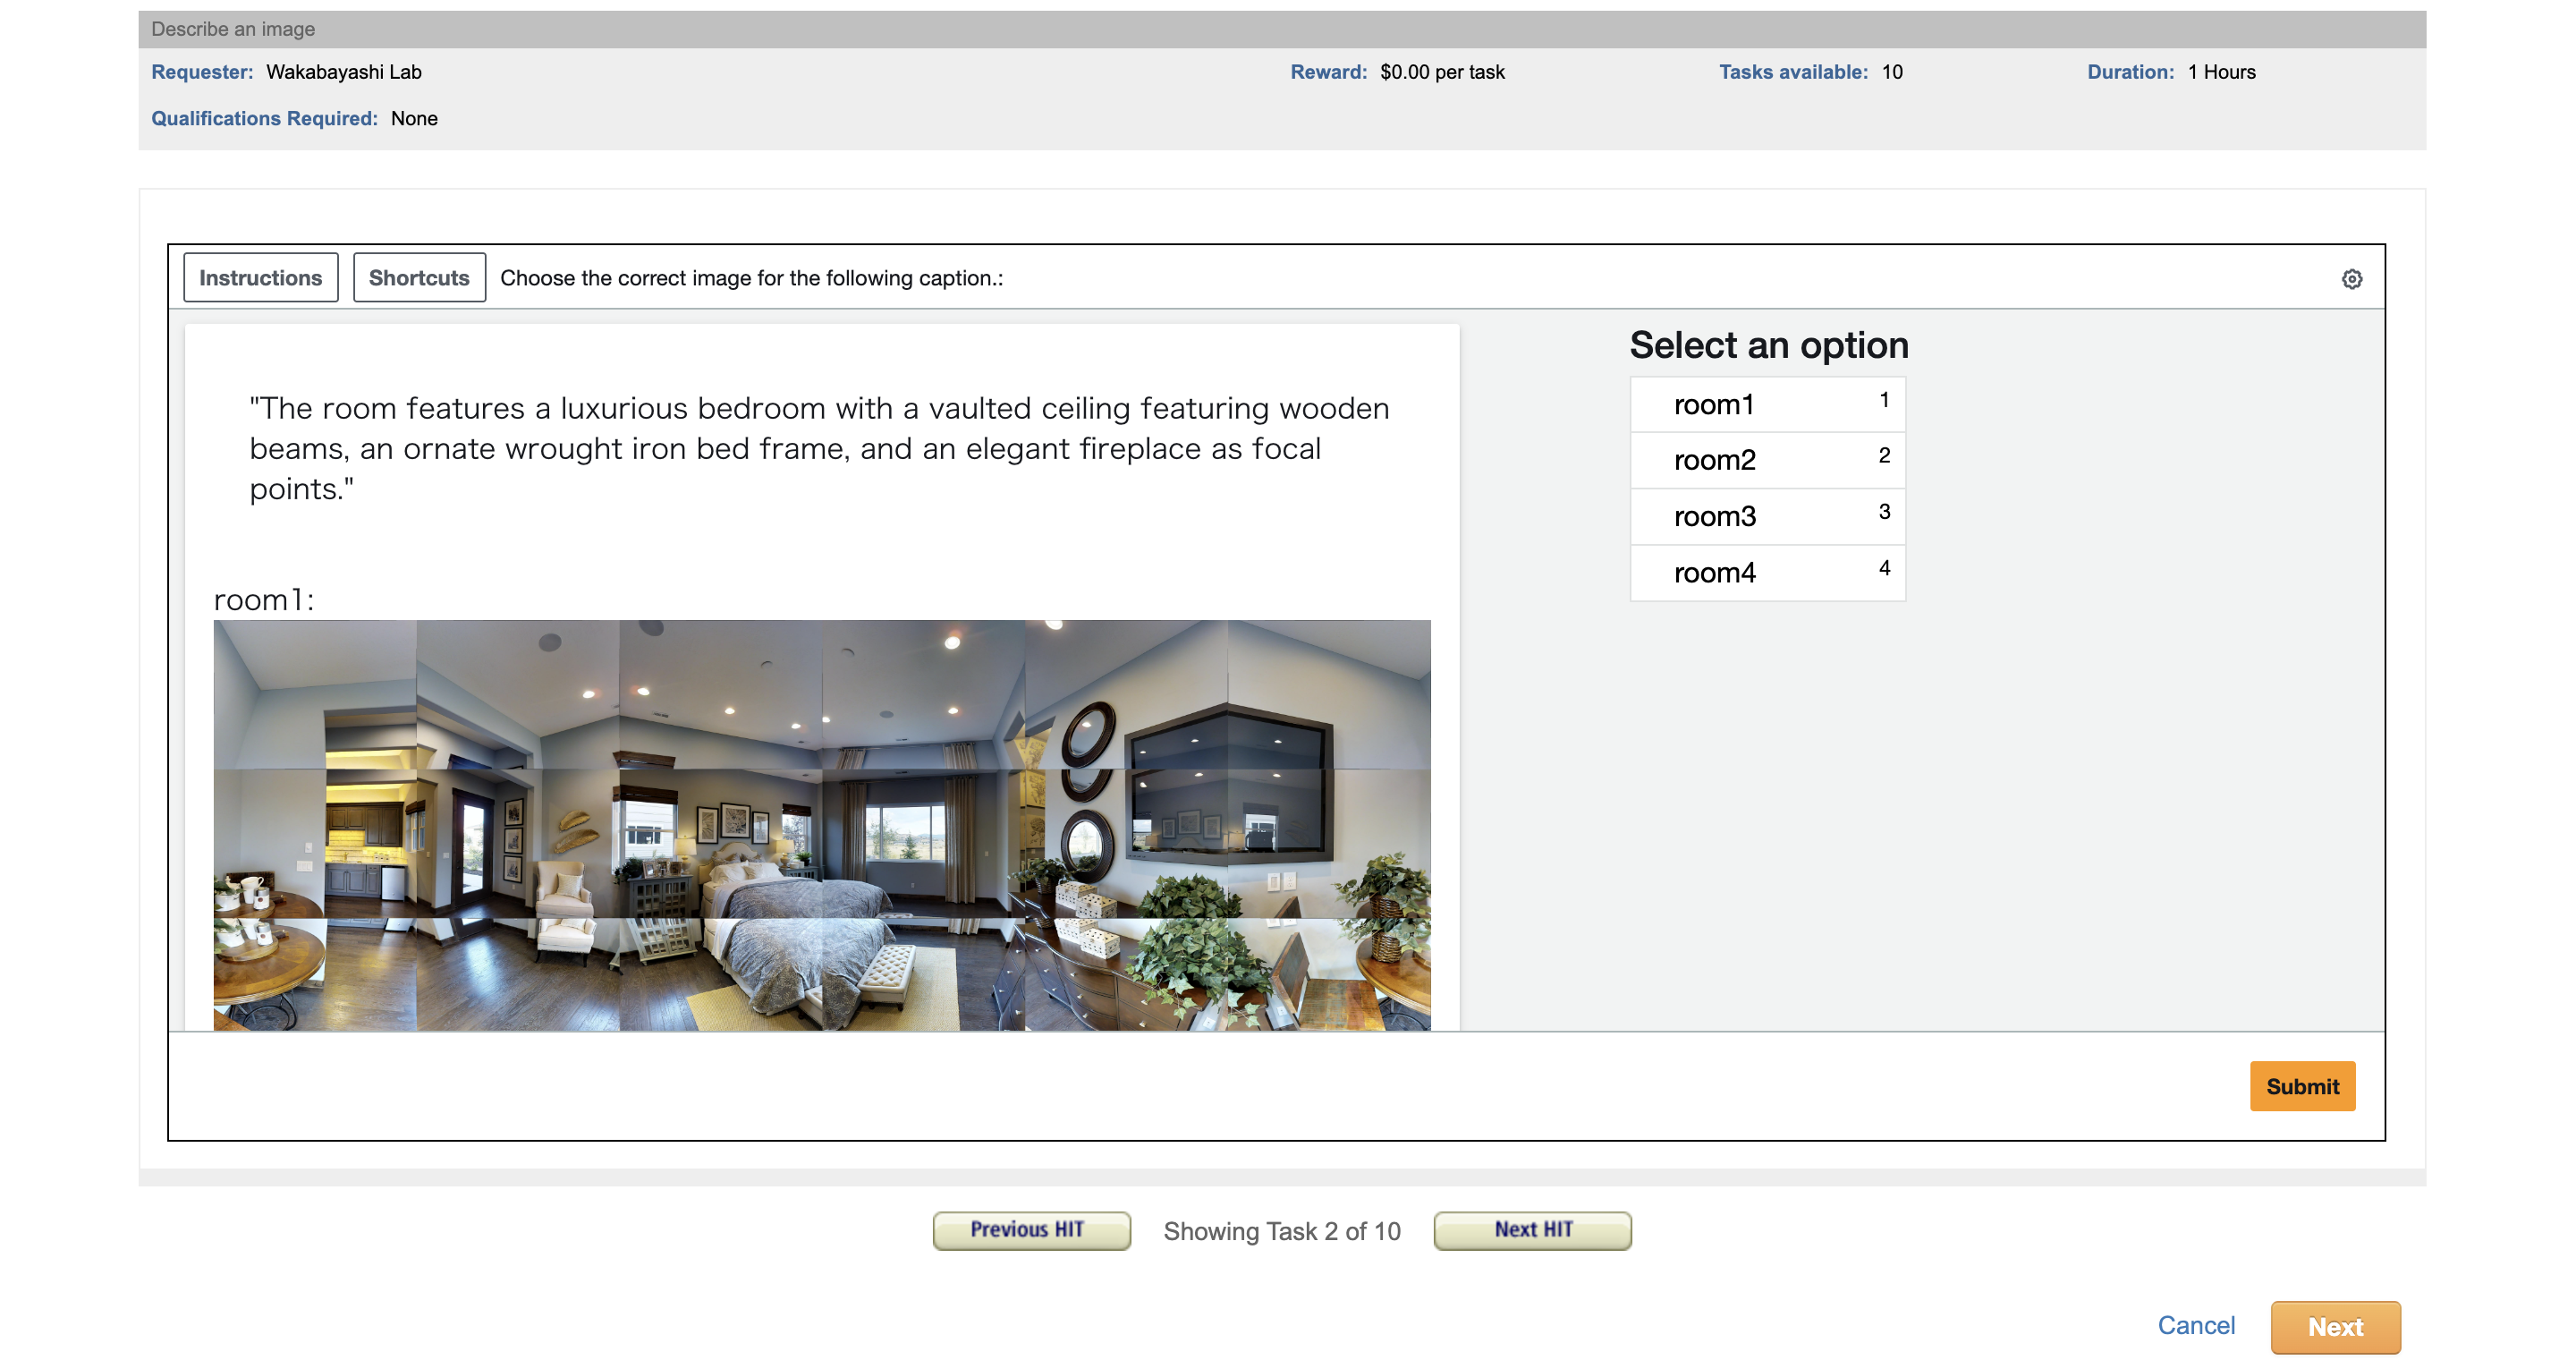
\includegraphics[width=\linewidth]{figures/amt.png}
  \caption{被験者に表示されるAMTタスクの例}
  \label{fig:amt_example}
\end{figure}

各手法ごとに,正解画像,ラベル,被りなくランダムに抽出した3枚の不正解画像の組み合わせによって作成したタスクを100回行う.

タスクの作成手順の詳細は以下の通りである.
\begin{enumerate}
  \item 10枚の画像と,各画像に対応する10個のラベルが手法によって生成される.
  \item ある画像が正解となるタスクを10タスク作成する.このとき,不正解となる3つの画像は,ランダムに被りなく抽出して組み合わせる.
  \item 10枚の画像それぞれに対して2の処理を行い,100通りの組み合わせのタスクを作成する.
\end{enumerate}

\subsection{比較手法}

実験では,4種類の方法で出力したラベルを使用して比較実験を行う.

ラベルの生成には以下の2つの手法を用いる.ベースライン手法との比較により,提案手法の評価を行う.
\begin{enumerate}
    \item ChatGPT(ベースライン手法)
    \item Pragmatic ChatGPT(PCG,提案手法)
\end{enumerate}

さらに,手法の一般性と実用性の評価のために,各手法で以下の2種類の出力方法でラベルを生成する.
\begin{enumerate}
  \item 通常出力(normal output):ラベル長に制限をかけずに出力
  \item 短出力(minimal output):ラベル長を10単語以内に制限し出力
\end{enumerate}

短出力では,図\ref{fig:limiting_prompt}に示すプロンプトをラベル出力処理部分に追加することで,ラベル長を10単語以内に収めるように制御する.

\begin{figure}[H]
\begin{mdframed}[linewidth=1pt]
Sentences must be output within 10 words.
\end{mdframed}
\caption{ラベル長に10単語以内の制限を設けるプロンプト}
\label{fig:limiting_prompt}
\end{figure}


ラベル長の制限は,手法の実用性を検証するために行う.無制限に長いラベルを生成することにより,理論上誤解を排除することは可能であるが,これは実用的ではない.従って,実験では,短いラベルによる誤解の可能性を低減できるかどうかについても検証を行う.これは,ラベルの長さが誤解可能性に与える影響を評価するために不可欠である.実際の応用においては,簡潔でありながら効果的なラベルが求められるため,短いラベルにおける性能評価は手法の実用性と妥当性を確認する上で重要である.

2手法それぞれで通常出力と短出力のラベルを生成し,合計4種類のラベル群のセットで被験者実験を行う.実験結果では,各手法で生成したラベル群の平均単語数もあわせて示す.

ベースライン手法によって生成されたラベルの例を図\ref{fig:label_example}に示す.

\begin{figure}[H]
\begin{mdframed}[linewidth=1pt]
Bright bedroom with large windows, modern decor, scenic view.
\end{mdframed}
\caption{出力されるラベルの例}
\label{fig:label_example}
\end{figure}

このようなラベルの集合を各手法で生成し実験に使用する.

実験で比較する各手法の名前と内容を箇条書きで説明する.

\begin{enumerate}
  \item ChatGPT
  \begin{itemize}
  \item ChatGPTを使用して,1枚の画像を入力して1つのラベルを出力する手法.以下のプロンプトを与えて,画像に対するラベルを出力する.
  \begin{figure}[H]
    \begin{mdframed}[linewidth=1pt]
      Generate a one-sentence description that captures only three features of the room you have provided.
    \end{mdframed}
    \caption{ベースライン手法で使用するプロンプト}
    \label{fig:baseline_prompt}
  \end{figure}
\end{itemize}
  
  \item Pragmatic ChatGPT(PCG)
  \begin{itemize}
    \item ChatGPTに「話し手モデル」「聞き手モデル」を導入し,ラベル改善サイクルを10回行う手法.
  \end{itemize}
    
  \item ChatGPT minimal
  \begin{itemize}
    \item ChatGPTに単語長10単語までの制約を加えた手法.\ref{fig:limiting_prompt}のプロンプトを,ラベル出力部分に追加する.,
  \end{itemize}
  
  \item Pragmatic ChatGPT minimal
  \begin{itemize}
    \item Pragmatic ChatGPTに単語長10単語までの制約を加えた手法.\ref{fig:limiting_prompt}のプロンプトを,ラベル出力部分に追加する.
  \end{itemize}
  
\end{enumerate}

\section{実験結果と考察}

\subsection{実験結果}

表\ref{tab:accuracy_result}は,手法ごとのAMTタスクの正答率と,タスクに使用したラベルの平均単語数を示している.
ChatGPTおよびChatGPT minimalがベースライン手法,Pragmatic ChatGPTおよびPragmatic ChatGPT minimalが提案手法である.

\begin{table}[H]
\centering
\begin{tabular}{lcc}
\hline
手法 & 正答率 & 平均単語数 \\
\hline
ChatGPT & 0.43 & 26.9 \\
Pragmatic ChatGPT & 0.40 & 20.7 \\
ChatGPT minimal & 0.31 & 7.5 \\
Pragmatic ChatGPT minimal & 0.33 & 8.1 \\
\hline
\end{tabular}
\caption{手法ごとのAMTタスクの正答率と平均単語数}
\label{tab:accuracy_result}
\end{table}

表\ref{tab:accuracy_result}より,ラベル長を制限した場合(ChatGPT minimalとPragmatic ChatGPT minimal),提案手法はベースライン手法の正答率を上回った.

ラベル長に制限が無い場合,提案手法はベースラインの正答率を下回った.

また,すべての比較手法において,平均単語数と正答率に若干の相関がみられた.

\subsection{考察}
本研究における提案手法は,ラベル長に制限がある場合に特に効果を発揮することが明らかになった.ラベル長が限定される状況では,画像の多様な特徴を一つのラベルで表現することには限界がある.この点において,提案手法はラベルの識別性を高める方向でのアプローチを取り,結果としてベースライン手法よりも高い正答率を達成した.このことから,短いラベルでの効果的な識別性の確保が提案手法の大きな強みであると言える.

一方で,ラベル長に制限がない場合の提案手法の性能については,いくつかの問題点が浮き彫りになった.無制限のラベル長では,各画像を包括的に表現することが可能であり,その場合,ラベルの顕著性を高めることがより重要となる.しかし,提案手法が依然として識別性の向上に重点を置いているため,この状況には適切に対応できていない.この結果,ベースライン手法と比較して,提案手法の正答率は低下することが観察された.

これらの考察に基づき,提案手法の改善策として,ラベルの顕著性と識別性のバランスを調整する機構の導入が提案される.具体的には,ラベルが長い場合は顕著性を,短い場合は識別性を優先させることで,ラベル長に応じた適切なラベル生成を行う.この改善により,ラベル長に制限がない状況においても,誤解可能性が低く,より効果的なラベル生成が期待できる.最終的には,この改善によって提案手法がベースライン手法と同等以上の効果を発揮する可能性がある.


% 結論
\chapter{おわりに}

本研究では,画像に対するラベル生成の問題を語用論的な観点から解決する試みを行った.特に,話し手モデルと聞き手モデルを導入し,その対話を通じてラベルの改善を図る新たなアプローチを提案した.

提案手法は,話し手モデルが作成したラベルを聞き手モデルが評価し,そのフィードバックに基づいてラベルを再生成するプロセスを繰り返すことで,より適切なラベルの生成を目指す.これにより,生成されたラベルが画像を一意に特定できるものであることが期待される.

また,本研究では生成したラベルの評価にAmazon Mechanical Turkを利用し,生成されたラベルが人間にとってどの程度理解しやすいかを検証した.その結果,提案手法によって生成されたラベルは,特にラベル長に制約がある場合において,ベースライン手法よりも優れた結果を示した.これは,提案手法がラベルの識別性を向上させることに重点を置いて設計されているためである.

今後の課題としては,より多様な画像やシーンに対するラベル生成の実施と,提案手法の汎用性の評価が挙げられる.また,聞き手モデルの評価基準やフィードバックの精度を向上させることも重要である.これらの課題を解決することで,本手法はさらに広範な応用が可能となると考えられる.

\chapter*{謝辞}
\addcontentsline{toc}{chapter}{\numberline{}謝辞}	% 目次で左詰めするなら \numberline{} を削除する.

本研究の一部は,JST CREST (\#JPMJCR22M2) の助成によって行われた.

\newpage

\addcontentsline{toc}{chapter}{\numberline{}参考文献}	% 目次で左詰めするなら \numberline{} を削除する.
\renewcommand{\bibname}{参考文献}

\bibliographystyle{junsrt}
\bibliography{reference}

\end{document}
